% Captions for the eight validation panels.
% Every number quoted below is read from results/ and was produced by the
% sweep that draws the corresponding subplot. Nothing here is asserted from
% the theory alone: where a claim is checked at one point and not across an
% axis, the caption says so.

\begin{figure*}[!htbp]
    \centering
    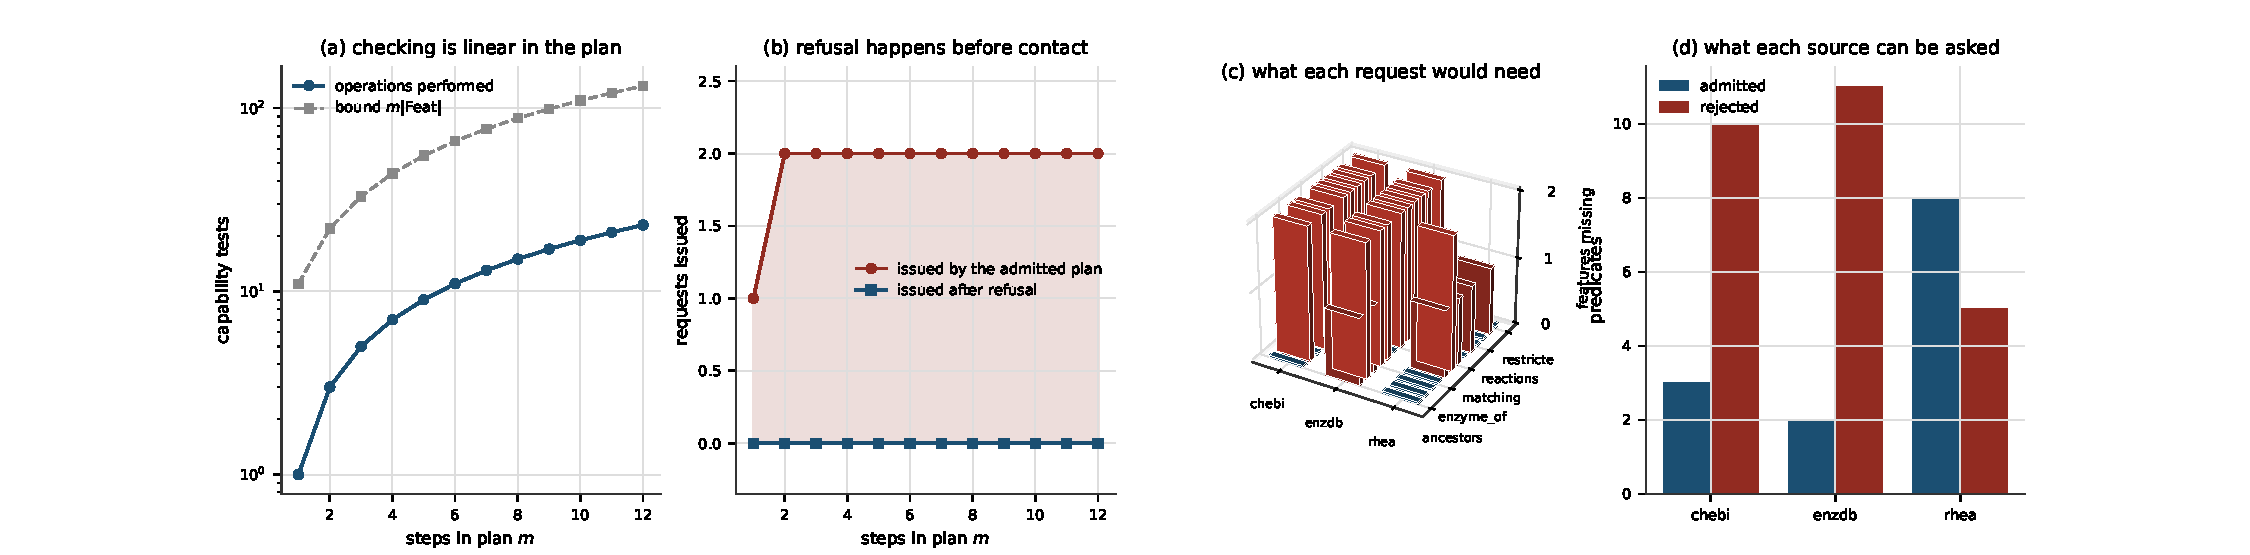
\includegraphics[width=\textwidth]{figures/panel_1_capability.pdf}
    \caption{\textbf{The static layer: checking is cheap, and refusal precedes contact.}
    Every quantity is produced by running the checker and the executor over parsed plans against a local registry of three sources and thirteen predicates; no request leaves the machine, so a request issued is a counter the executor incremented and not an estimate.
    (\textbf{A})~Operations performed by the check against plan length for $m = 1 \dots 12$. The measured count is exactly $2m-1$ against a declared bound of $11m$, one per feature; the check is linear in $m|\mathrm{Feat}|$ as \Cref{thm:static} requires, and the gap between the two lines is the constant the bound does not attempt to be tight about.
    (\textbf{B})~Requests actually issued, at every plan length rather than at one. The upper series is what the well-capable plan spends and the lower is what the same plan spends once its first step is pointed at a source that cannot answer it; \Cref{cor:refuse-before-contact} pins the lower series at exactly $0$ for all twelve lengths. The upper series is $1$ at $m=1$ and then \emph{saturates at $2$}: the chain starves after its second step, so the saving does not grow with $m$, and this caption declines to draw a curve that would suggest it does.
    (\textbf{C})~For each of $39$ source--predicate pairs, the number of declared features the request would still need. The height is the integer the checker computed, so the bars are drawn as bars: a surface would interpolate a step function through values it never takes. Zero (blue) means admissible, and $2$ (red) means two features short.
    (\textbf{D})~The same $39$ pairs resolved into admitted and rejected counts per source. The three sources are unequal by construction --- \texttt{chebi} admits $3$ of $13$, \texttt{enzdb} $2$, \texttt{rhea} $8$ --- and it is that inequality, not the checker, that decides which plans can be written at all. Under \Cref{rem:honesty-assumption} this figure records what each source \emph{declares}; an over-declaration would be invisible here, which is the asymmetry the prototype cannot test away.}
    \label{fig:panel1}
\end{figure*}

\begin{figure*}[!htbp]
    \centering
    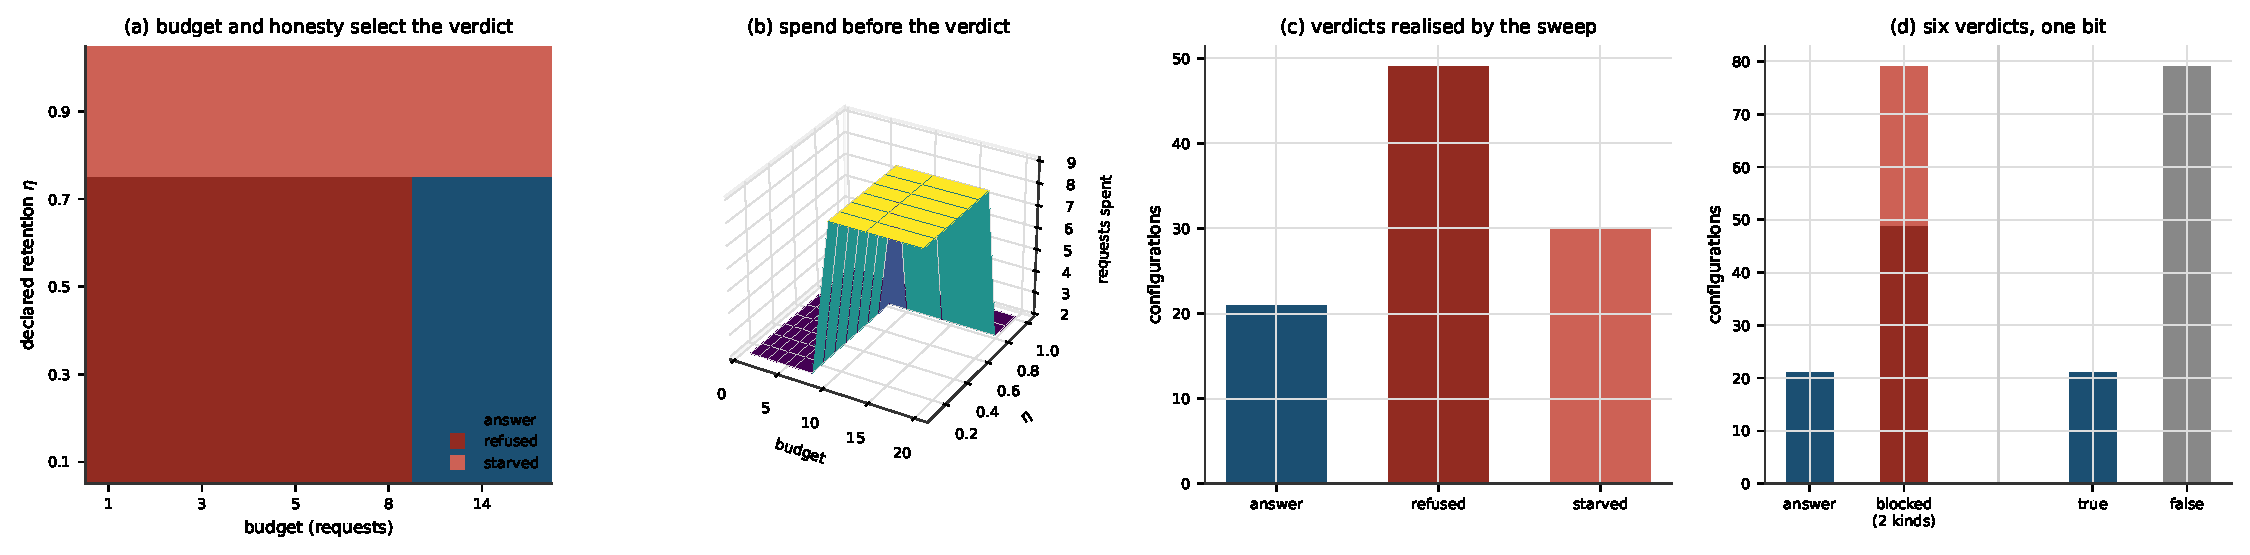
\includegraphics[width=\textwidth]{figures/panel_2_verdicts.pdf}
    \caption{\textbf{The verdict layer: six outcomes, one observable bit.}
    A $10 \times 10$ sweep executes the same plan across ten budgets $B \in \{1,2,3,4,5,6,8,10,14,20\}$ and ten declared-honesty levels $\eta \in \{0.1 \dots 1.0\}$, giving $100$ executed plans; the verdict in each cell is the one the ordered rules (R1)--(R6) of \Cref{thm:six} returned.
    (\textbf{A})~The verdict attained in each cell. Of the $100$ executions, $21$ answer, $49$ refuse and $30$ starve, and \texttt{answer} appears only at budgets $10$, $14$ and $20$. The budget axis is geometric and is labelled by value rather than by position, because drawing $\{1 \dots 20\}$ on a linear extent would misstate where the transition sits.
    (\textbf{B})~Requests spent before the verdict was returned. The spend is single-valued within each verdict --- $9.0$ for \texttt{answer}, $2.0$ for \texttt{refused}, $2.0$ for \texttt{starved} --- so the plot has three levels and not a cloud. The \texttt{refused} here is \emph{budget exhaustion} and costs $2.0$ requests; it is not the static ill-capability refusal of \Cref{fig:panel1}(B), which costs $0$. The two share a name and nothing else, and no figure in this paper should be read as reconciling them.
    (\textbf{C})~The verdicts the sweep realises from named plans, with the blocker each carries. All six of \Cref{thm:six} occur, with blockers \texttt{model}, \texttt{engine}, \texttt{corpus} and \texttt{budget} for the four blocked kinds and none for the two that are not blocked.
    (\textbf{D})~The collapse of \Cref{cor:onebit}. Across the sweep, $21$ executions carry the true bit and $79$ the false one; the five non-\texttt{answer} kinds are distinct verdicts with distinct blockers and identical payload size $0$, so a caller reading only success or failure cannot separate them. \Cref{prin:verdict} is what makes this a collapse rather than a loss: a payload accompanies \texttt{answer} alone, so there is nothing else for the bit to have carried.}
    \label{fig:panel2}
\end{figure*}

\begin{figure*}[!htbp]
    \centering
    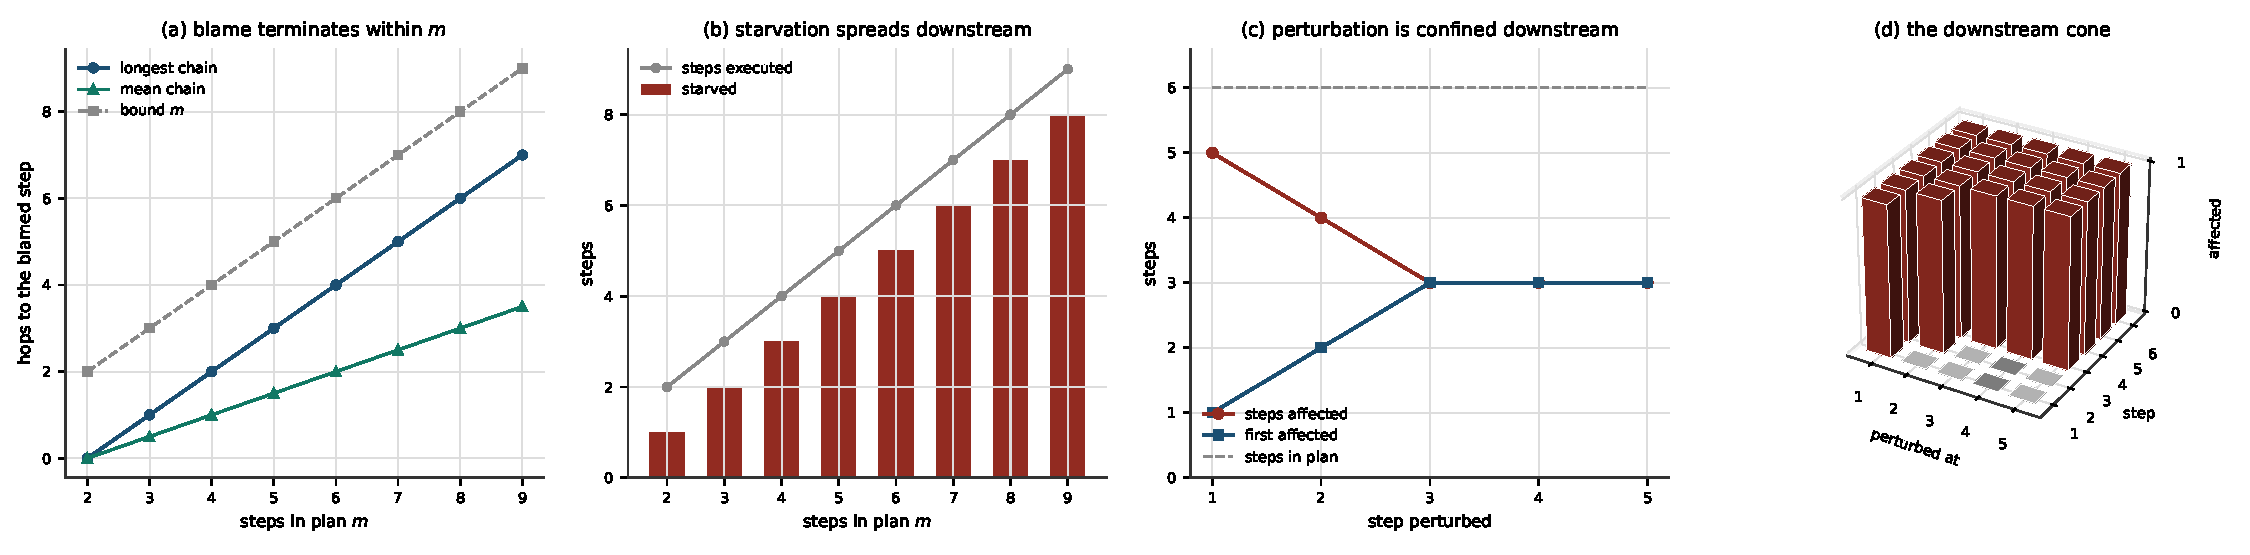
\includegraphics[width=\textwidth]{figures/panel_3_blame.pdf}
    \caption{\textbf{Blame: it terminates, and it only ever runs downstream.}
    Plans of length $m = 2 \dots 9$ are executed with a starving first step and the blame chain is walked to its root; hop counts are traversal lengths recorded during the walk.
    (\textbf{A})~The longest and mean blame chain against plan length, with the $m$-hop bound of \Cref{prop:blame}. The measured maximum is exactly $m-2$ and the mean exactly $(m-2)/2$, both strictly under the bound at every length. The mechanism is that positions strictly decrease along a chain, so termination is not a budget but an arithmetic fact.
    (\textbf{B})~How much of each plan starves. Exactly $m-1$ of $m$ steps starve at every length: one step fails and every step below it inherits the failure, which is \Cref{prop:starve-reachable} read off the executed plans rather than argued.
    (\textbf{C})~A single perturbation applied at each position of one six-step plan. Perturbing step $1$ affects $5$ steps and first bites at $1$; perturbing steps $3$, $4$ or $5$ affects $3$ and first bites at $3$. The two series diverge because the first affected step is not the perturbed step once the perturbation lands inside a region already downstream of a common dependency.
    (\textbf{D})~The reachability cone the previous panel summarises: for each perturbation position $i$, which steps $j$ can be affected. The filled cells lie on or below the diagonal only --- nothing upstream of the perturbation is ever touched. That null could have failed: the sweep records reachability as computed from the executed dependency graph, not from a triangular structure that would make the shape true by construction.}
    \label{fig:panel3}
\end{figure*}

\begin{figure*}[!htbp]
    \centering
    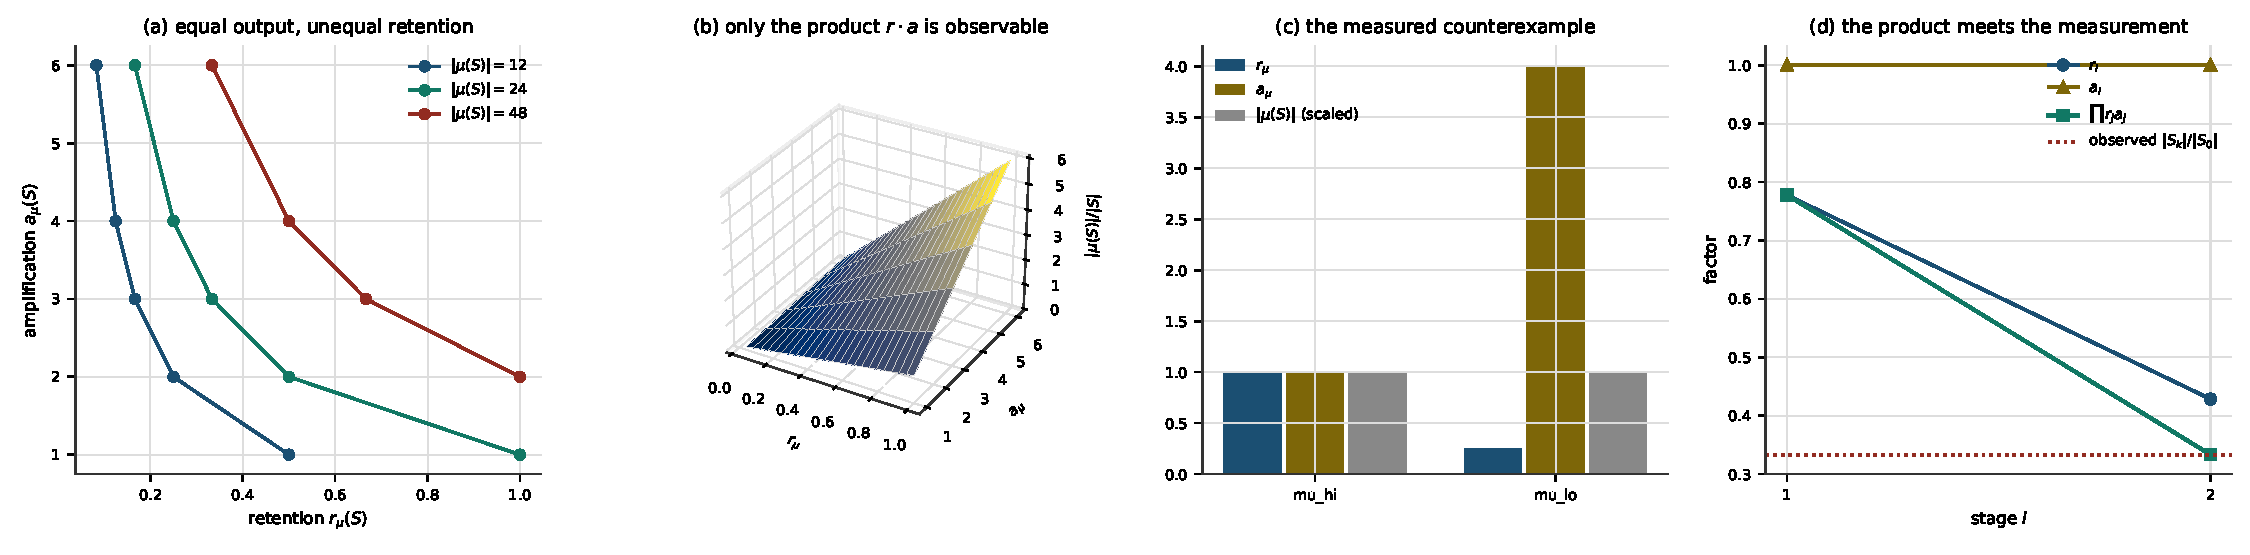
\includegraphics[width=\textwidth]{figures/panel_4_retention.pdf}
    \caption{\textbf{Retention and amplification are independent, and output size sees only their product.}
    Retention $r_\mu(S) = |S \cap \operatorname{dom}\mu|/|S|$ and amplification $a_\mu(S) = |\mu(S)|/|S \cap \operatorname{dom}\mu|$ are computed on realised sets from executed maps; $144$ cells sweep the pair.
    (\textbf{A})~Iso-cardinality families: every point on one curve produces the same $|\mu(S)|$. At $|\mu(S)| = 12$ the retention ranges over $0.083$--$0.5$ while the amplification ranges over $1$--$6$, a spread of $6.0$; at $|\mu(S)| = 24$ the same spread holds at retentions $0.167$--$1.0$. Equal output size is compatible with a sixfold difference in how much of the input survived.
    (\textbf{B})~The observable ratio $|\mu(S)|/|S| = r \cdot a$ over the $(r, a)$ plane, with the level curves at $0.5$, $1$ and $2$ projected onto the floor. The surface is a product, so its level sets are hyperbolae and every point on one is indistinguishable from the outside: this is exactly what \Cref{prop:cardinality-uninformative} claims cannot be undone by measuring $|\mu(S)|$ more carefully.
    (\textbf{C})~The measured counterexample, executed rather than constructed on paper. Two maps over the same $8$-element input both emit $8$ identifiers; \texttt{mu\_hi} has $r = 1.00$, $a = 1.0$ and \texttt{mu\_lo} has $r = 0.25$, $a = 4.0$ --- a retention ratio of $4.0$ at identical output cardinality and identical product $1.0$. The grey series is output size, scaled, and its flatness is the point.
    (\textbf{D})~The factorisation of \Cref{thm:retention}(a) along a measured two-stage chain. Stage retentions are $0.778$ and $0.429$ with both amplifications $1.0$; the running product reaches $0.333$ and the observed $|S_k|/|S_0|$ is $0.333$ to the last recorded digit. This chain is \emph{not} injective, and part~(a) holds anyway --- which is why (a) is stated unconditionally and (b) and (c) are not.}
    \label{fig:panel4}
\end{figure*}

\begin{figure*}[!htbp]
    \centering
    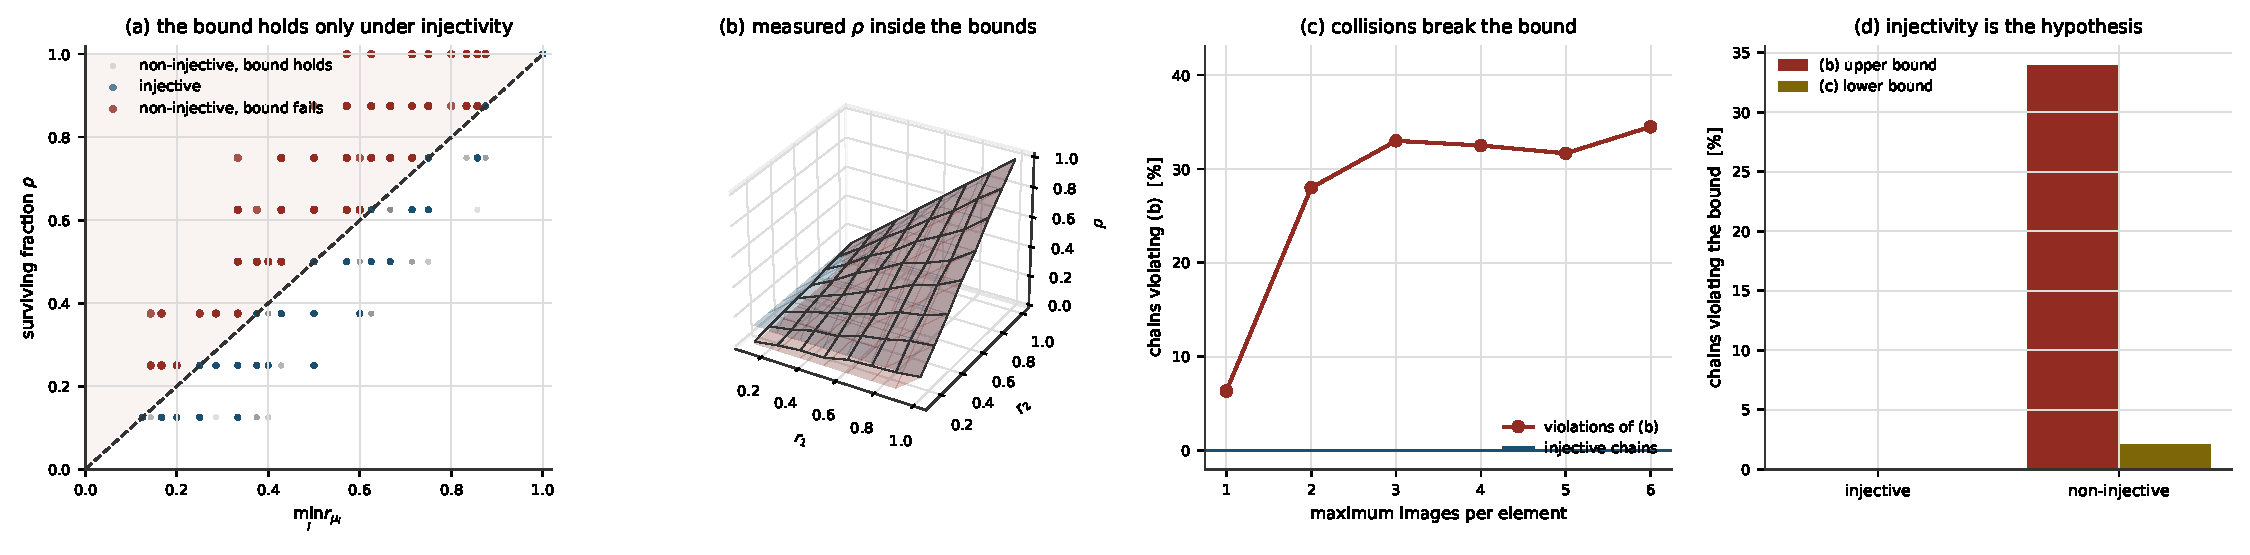
\includegraphics[width=\textwidth]{figures/panel_5_bounds.pdf}
    \caption{\textbf{Injectivity is the hypothesis, not a convenience of the proof.}
    Chains are drawn over $8$-element supports at domain probability $0.8$ and at most $3$ images per element; injective chains are constructed rather than rejection-sampled, so the two populations are matched in everything except the property under test.
    (\textbf{A})~Surviving fraction $\rho$ against $\min_i r_{\mu_i}$ for $1200$ injective and $1158$ non-injective chains. Every injective chain lies on or below the diagonal, as \Cref{thm:retention}(b) requires. Of the non-injective chains, $315$ ($27.2\%$) lie strictly above it and are drawn alone in the alarm colour; the remainder are greyed, because a non-injective chain that happens to respect the bound is not evidence either way. The shaded wedge above the diagonal is the region the theorem forbids under its hypothesis, and it is populated.
    (\textbf{B})~Measured $\rho$ (wireframe) between the upper bound of (b) and the lower bound of (c) over an $8 \times 8$ grid in $(r_1, r_2)$, $64$ cells. The measured value touches the upper sheet in $8$ cells and never crosses either sheet. The vertical separation reaches $0.253$ above and $0.247$ below, and per \Cref{rem:bounds-gap} that separation is not slack to be tightened: the two bounds answer different questions.
    (\textbf{C})~Violation rate of (b) against how non-injective the chain is, $600$ trials at each image cap. At one image per element the rate is $6.3\%$ --- \emph{not} zero, because capping images at one does not by itself forbid two elements sharing an image --- rising to $28$--$34.5\%$ once two or more images are allowed. The flat blue line is the constructed-injective control at exactly $0$; without it the red curve would have no floor to be read against, and the $6.3\%$ would look like noise rather than residual collision.
    (\textbf{D})~Both bounds against both populations at $n = 5000$ each. Injective chains violate the upper bound $0$ times and the lower bound $0$ times; non-injective chains violate the upper $1694$ times ($33.9\%$) and the lower $102$ times ($2.0\%$). The four bars are the whole of \Cref{rem:injectivity-needed}: two zeros that could have been non-zero, beside two non-zeros that could have been zero.}
    \label{fig:panel5}
\end{figure*}

\begin{figure*}[!htbp]
    \centering
    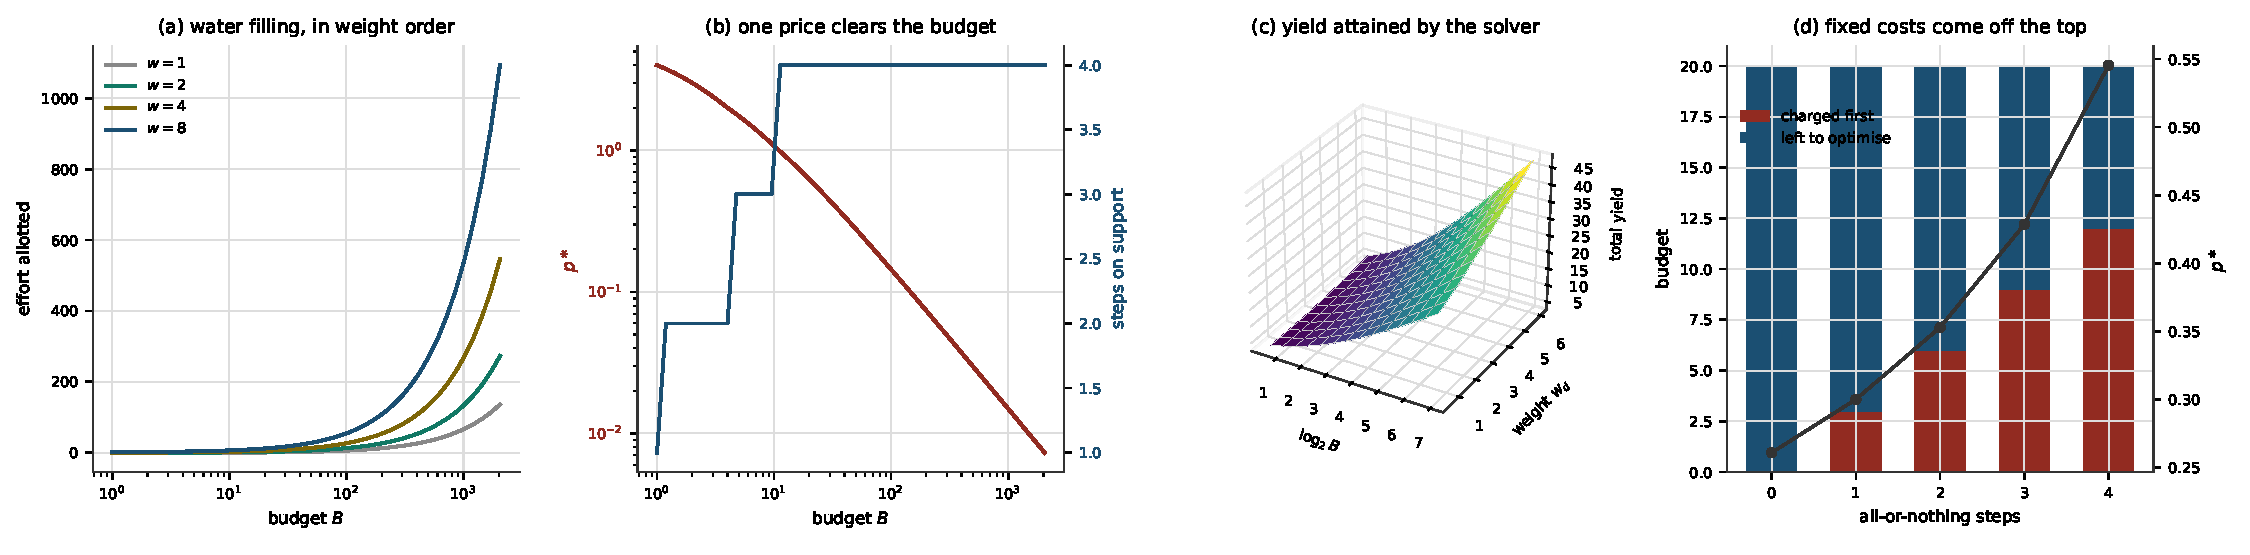
\includegraphics[width=\textwidth]{figures/panel_6_allocation.pdf}
    \caption{\textbf{Allocation: one shadow price clears the budget, and fixed costs are charged before it.}
    The allocator of \Cref{thm:allocation} is solved at $45$ budgets spanning $B = 1$ to $2048$ over four steps of weight $1, 2, 4, 8$; every plotted effort is a solved primal variable and every price a solved dual.
    (\textbf{A})~Effort allotted to each step as the budget grows, on a logarithmic budget axis. Steps enter in weight order and not together: at $B = 1$ only the heaviest step is funded, at $B = 4$ two are, and all four are on support from $B = 16$ upward. Water filling is visible as the staggered onset, which no single-budget summary of the allocator would show.
    (\textbf{B})~The shadow price $p^\ast$ and the size of the support against the budget, with the price on logarithmic axes. $p^\ast$ falls monotonically from $4.00$ to $7.31 \times 10^{-3}$ across the sweep while the support rises from $1$ to $4$ and then stops; the kinks in the price are exactly the budgets at which a step enters. The maximum KKT residual over all $45$ solves is $1.11 \times 10^{-16}$, which is machine epsilon rather than a tolerance that was chosen.
    (\textbf{C})~Total yield over budget and the weight of the fourth step, $168$ solved allocations. The surface is concave in $\log_2 B$ at every weight, and the yield rises from $5.55$ at $B = 1$ to $97.34$ at $B = 2048$.
    (\textbf{D})~What happens when steps carry an all-or-nothing or fixed cost: those are charged first and the optimiser gets what remains. As the number of such steps goes $0 \to 4$, the charged-first amount rises $0 \to 12$ and the optimised budget falls $20 \to 8$; the price rises with it, $0.261 \to 0.545$. The rising price is the honest report that the same total budget buys strictly less once part of it is spent before the optimisation can see it.}
    \label{fig:panel6}
\end{figure*}

\begin{figure*}[!htbp]
    \centering
    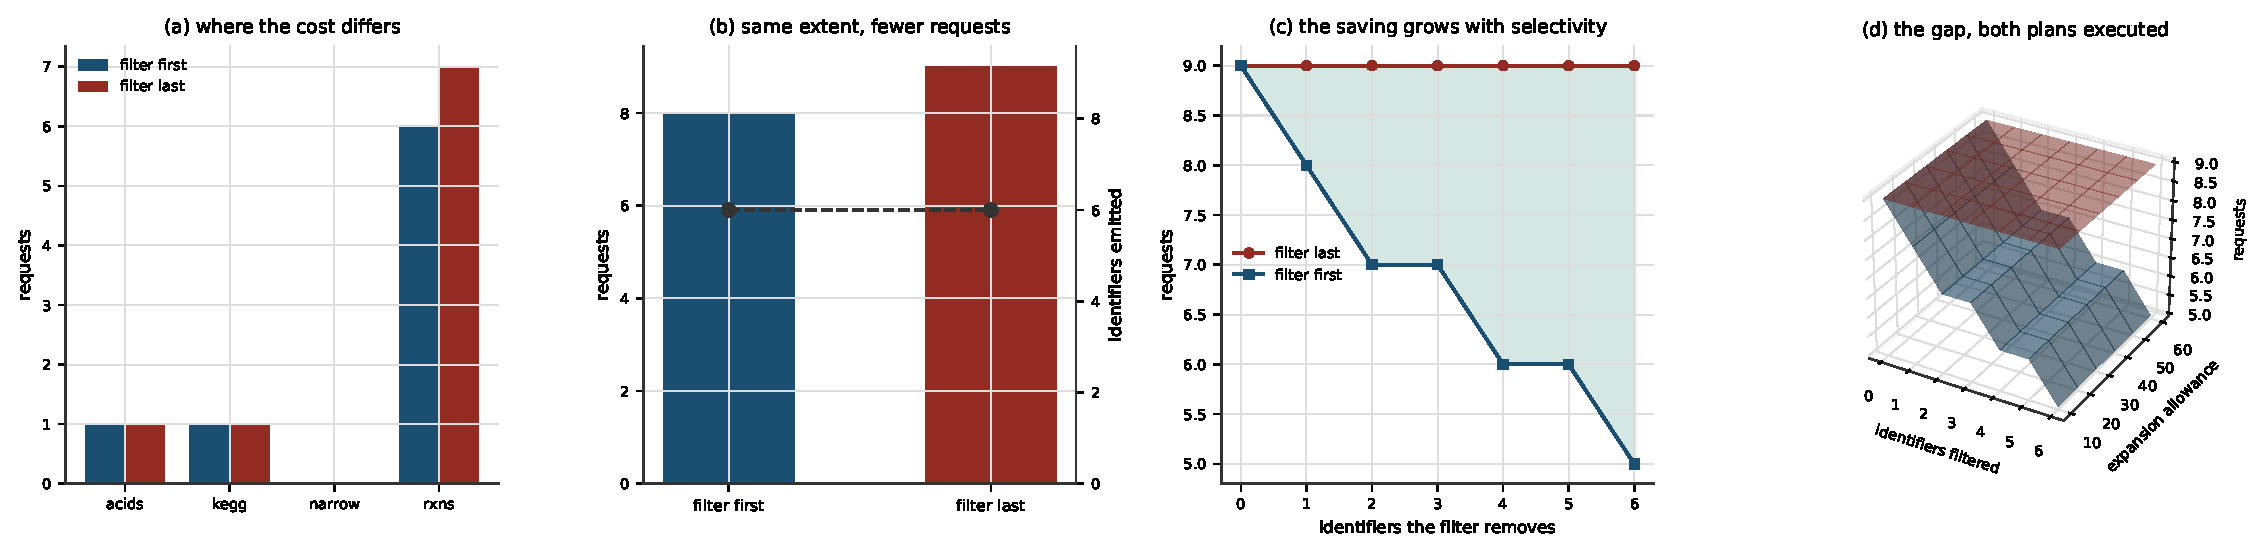
\includegraphics[width=\textwidth]{figures/panel_7_ordering.pdf}
    \caption{\textbf{Ordering: the same extent at a different price.}
    Two plans containing the same four steps in two orders are parsed, checked and executed; every request count below is a counter the executor incremented, and the closed-form cost model that also exists in the sweep is deliberately not plotted anywhere in this figure.
    (\textbf{A})~Requests spent per step by the two orderings. The steps \texttt{acids} and \texttt{kegg} cost $1$ each in both plans; the difference is entirely in the last two, where filtering first makes \texttt{rxns} cost $6$ and filtering last makes it cost $7$. No step is cheaper under the worse ordering, which is what makes the comparison a saving rather than a trade.
    (\textbf{B})~Totals. Both plans emit the same six identifiers --- \texttt{RHEA:100} through \texttt{RHEA:105}, set-equal and not merely equal in count --- at $8.0$ and $9.0$ requests. The dashed coverage line is flat by measurement, and if it were not, the request comparison beside it would mean nothing.
    (\textbf{C})~Both orderings executed as the filter is made more selective, at the expansion allowance the shipped plans use. Requests under filter-last stay pinned at $9.0$ regardless of selectivity, while filter-first falls $9.0 \to 5.0$ as the filter removes $0 \to 6$ identifiers. The measured series has step structure --- flat across $2 \to 3$ and again across $4 \to 5$ --- which a smooth cost model would have drawn as a straight line.
    (\textbf{D})~The two measured surfaces over filter size and expansion allowance, $42$ executed plans. The sheets touch at zero selectivity and separate as the filter bites, with a maximum measured saving of $4$ requests. Coverage was checked equal in all $42$ cells; per \Cref{rem:reorder-cost} the saving is a cost difference and never an extent difference, and the sweep records no cell where that failed.}
    \label{fig:panel7}
\end{figure*}

\begin{figure*}[!htbp]
    \centering
    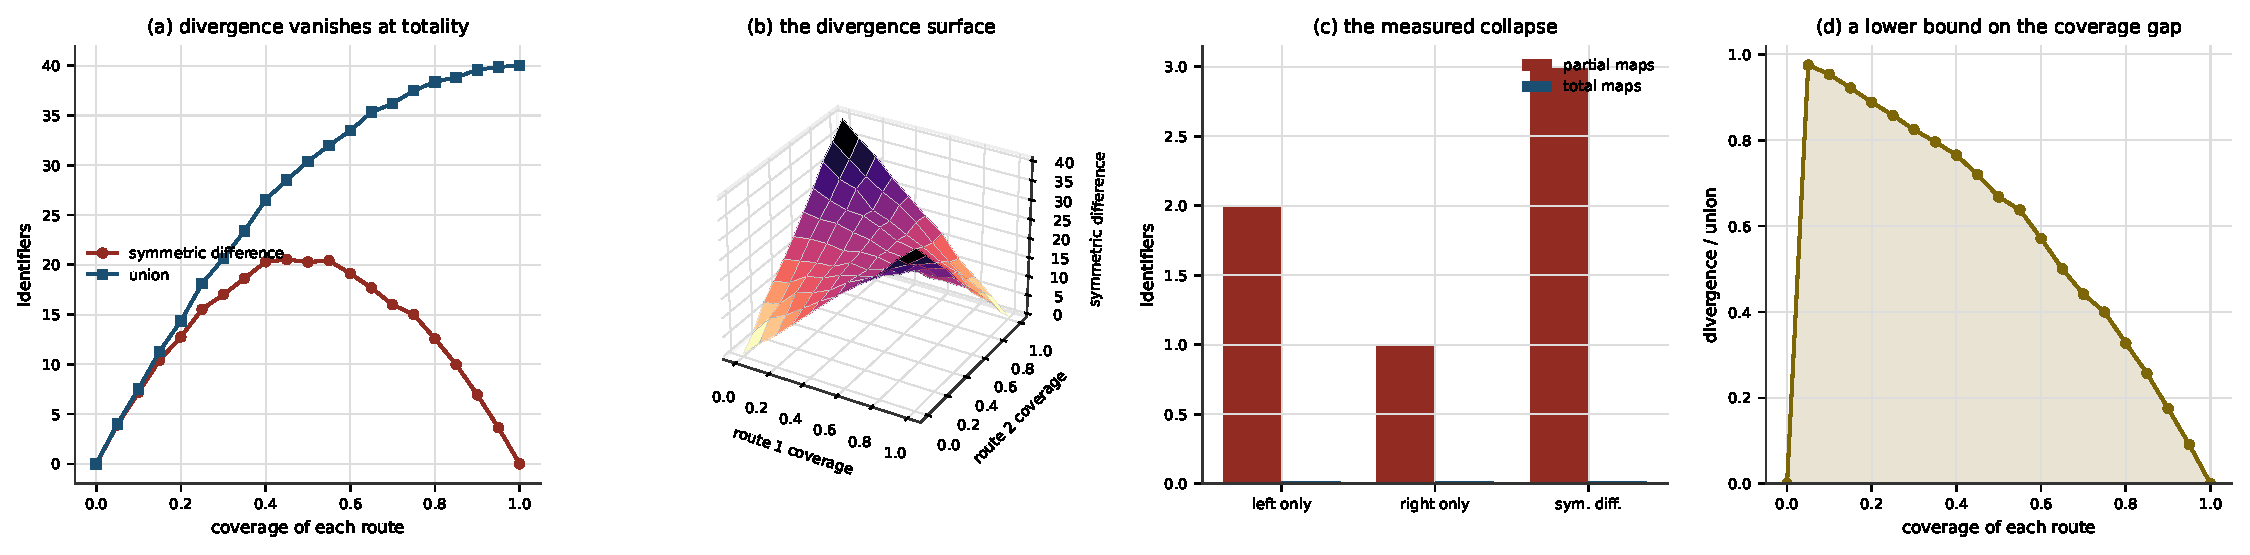
\includegraphics[width=\textwidth]{figures/panel_8_routes.pdf}
    \caption{\textbf{Two routes: divergence is a coverage gap, and it collapses under totality.}
    Two independent routes between the same endpoints are resolved at controlled coverage; the symmetric difference is computed on realised identifier sets, and the interpretation of \Cref{thm:route-extent}(b) is fixed before any number is read.
    (\textbf{A})~Symmetric difference and union as both routes are made more total, $21$ coverage levels. The divergence rises to a maximum of $20.3$ identifiers near coverage $0.4$ and then falls back to exactly $0$ at coverage $1.0$, while the union climbs monotonically to $40$. The non-monotone shape is the substance: divergence is small when both routes see little and small again when both see everything, and it is largest in between.
    (\textbf{B})~The same quantity over independent coverage for the two routes, $121$ cells. The surface carries a ridge along the diagonal, peaking at $20.6$ where both routes cover half. Only $2$ of $121$ cells are exactly zero, and both lie at the corners where the two routes agree trivially.
    (\textbf{C})~The measured collapse from the fixture. With partial maps the routes differ on $3$ identifiers --- $2$ resolved only by the direct route, $1$ only by the indirect --- out of a union of $8$. With both maps made total, all three counts are exactly $0$; the thick rules mark those measured zeros so they cannot be mistaken for an absent series.
    (\textbf{D})~Divergence as a fraction of the union, which is the form in which the claim is actually usable. The fraction peaks near $0.6$ and returns to $0$ at totality. Per \Cref{thm:route-extent}(b) this is a \emph{lower} bound on the correspondences at least one route fails to resolve, and not a count of errors: neither route contradicts the other anywhere in this sweep, and nothing here licenses reading a divergence as one route being wrong.}
    \label{fig:panel8}
\end{figure*}
